\documentclass[aps,twocolumn]{revtex4-1}

\usepackage{amsfonts}
\usepackage{amsmath}
\usepackage{geometry}
\usepackage{xcolor}
\usepackage{graphicx}
%\usepackage[subfolder,cleanup]{gnuplottex}
%\usepackage{amsthm}
%\usepackage{enumitem}
%\usepackage{wrapfig}
%\usepackage{subcaption}
%\usepackage{hyperref}
\usepackage{tikz}

% Nicer brackets for operators
\let\originalleft\left
\let\originalright\right
\renewcommand{\left}{\mathopen{}\mathclose\bgroup\originalleft}
\renewcommand{\right}{\aftergroup\egroup\originalright}

% Math operators
\providecommand{\bigO}[1]{\ensuremath{\mathop{}\mathopen{}\mathcal{O}\mathopen{}\left(#1\right)}}

% Macros
\newcommand{\diff}[3][\hspace{-0.5pt}]{\frac{\textrm{d}^{#1}#2}{\textrm{d}{#3}^{#1}}}
\newcommand{\pdiff}[3][\hspace{-0.5pt}]{\frac{\partial^{#1}#2}{\partial{#3}^{#1}}}
\newcommand{\df}{\, \textrm{d}}
%\newcommand{\eps}{\varepsilon}

% Row colouring in tables
%\usepackage[table]{xcolor}
%\rowcolors{2}{gray!25}{white}

% Margin size
\newgeometry{margin=2cm}

% Reference style
%\bibliographystyle{ieeetr}

\begin{document}

\title{Predicting NCAA March Madness 2019 with SpringRank}
\author{Brady Metherall}
\noaffiliation
\date{16 March, 2020}

\maketitle

\begin{figure}[tbp]
	\centering
	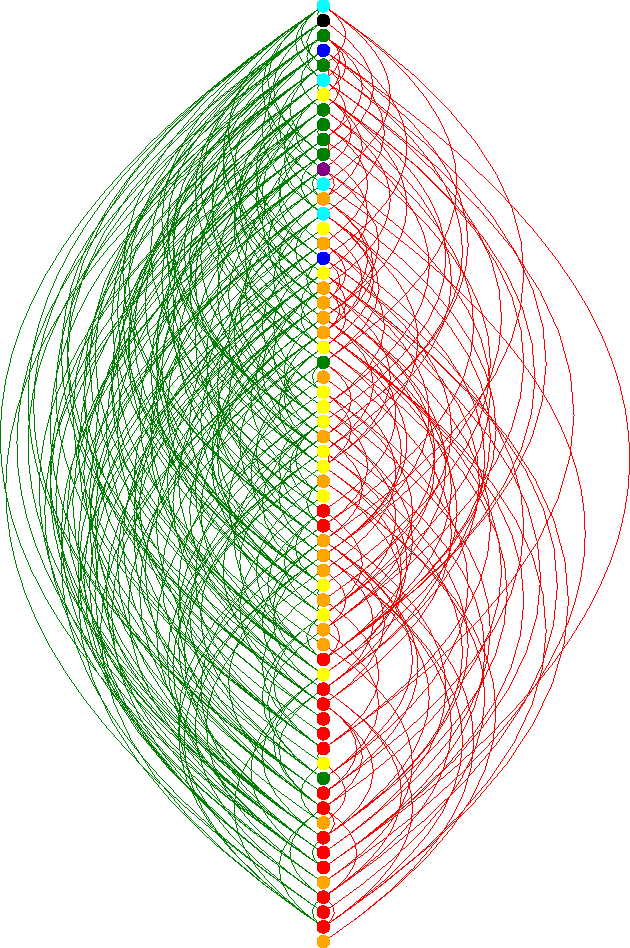
\includegraphics[width=0.75\columnwidth]{Heirarchy}
	\caption{}
	\label{fig:heir}
\end{figure}

\begin{figure}[tbp]
	\centering
	\begin{tikzpicture}
		\centering
		\node[anchor=south west,inner sep=0] at (0,0) {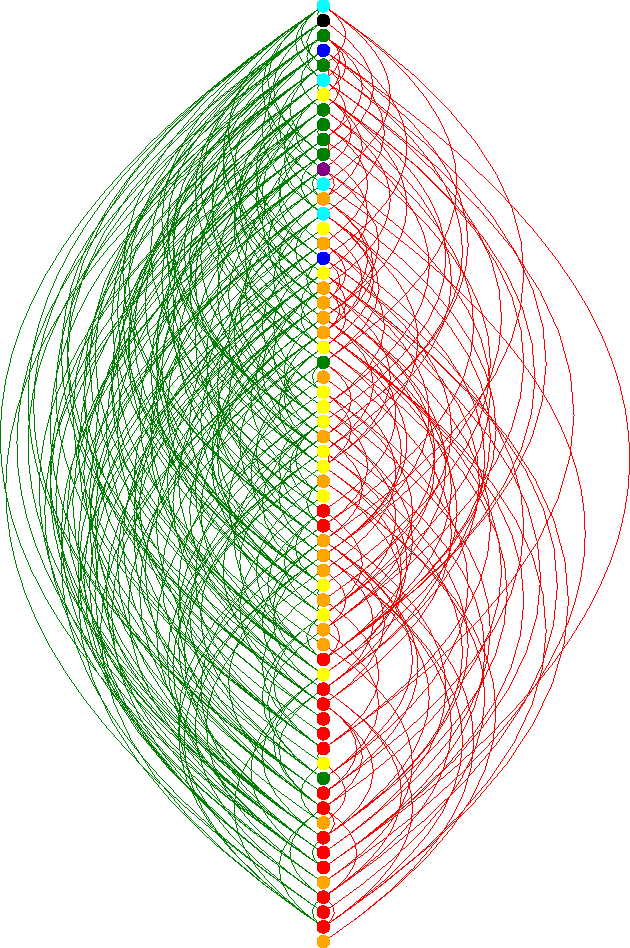
\includegraphics[width=0.66\columnwidth]{Heirarchy}};

		\fill[fill = black] (0.4,1) circle (0.6mm);
		\fill[fill = purple] (0.4,0.667) circle (0.6mm);
		\fill[fill = blue] (0.4,0.333) circle (0.6mm);
		\fill[fill = cyan] (0.4,0) circle (0.6mm);

		\node[anchor = west] at (0.5,1) {\scriptsize Winner};
		\node[anchor = west] at (0.5,0.667) {\scriptsize Runner-up};
		\node[anchor = west] at (0.5,0.333) {\scriptsize Final four};
		\node[anchor = west] at (0.5,0) {\scriptsize Elite eight};

		\fill[fill = green] (4.4,1) circle (0.6mm);
		\fill[fill = yellow] (4.4,0.667) circle (0.6mm);
		\fill[fill = orange] (4.4,0.333) circle (0.6mm);
		\fill[fill = red] (4.4,0) circle (0.6mm);

		\node[anchor = west] at (4.5,1) {\scriptsize Sweet 16};
		\node[anchor = west] at (4.5,0.667) {\scriptsize Round of 32};
		\node[anchor = west] at (4.5,0.333) {\scriptsize Round of 64};
		\node[anchor = west] at (4.5,0) {\scriptsize Did not qualify};
	\end{tikzpicture}
	\caption{}
	\label{fig:heir}
\end{figure}


colour = {1: 'black', 2: 'purple', 4: 'blue', 8: 'cyan', 16: 'green', 32: 'yellow', 64: 'orange', -1: 'red'}

\cite{debacco}

\cite{wirth}

\cite{vanderkam}

\bibliography{Ref}

\end{document}
